En este capítulo se explicara una guía detallada paso a paso de como crear y desplegar un LMS con esta aplicación. En los capítulos siguientes se entrará en más detalle con respecto a la toma de decisiones en el diseño y como se ha logrado implementar todo la aplicación.

\section{Instalar node y un instalador de paquetes de JS}

Lo primero será descargar lo necesario para crear una aplicación que use javascript, en este caso, se deberá instalar \verb|node| \cite{nodejs}, con el siguiente link \cite{node-install} para Windows y Mac y en caso de usar una distribución de Linux el siguiente \cite{node-install-linux}. Esta instalación de normal ya trae incluido el instalor de paquetes npm, el cual se usará para los posteriores ejemplos. Si se desea instalar otro como \verb|pnmn| \cite{pnpm} o \verb|yarn| \cite{yarn}, habría que seguir la propia instalación de cada uno.

\section{Crear un Classroom de GitHub}

Esta aplicación esta centrada en la filosofía de enseñanza de GitHub, es por esto que lo primero que se deberá hacer es crear un GitHub Classroom, una herramienta para la enseñanza de GitHub. Para empezar se debera crear una cuenta de GitHub como se especifica aquí \cite{github-account}. Tras haber creado una cuenta de GitHub se podrá proceder a crear el Classroom, siguiendo la siguiente guía \cite{github-classroom-create}.

\section{Empezar una LMS con {\tt AdAstra}: create-adastra-lms}

Para empezar a usar el generador de LMS se deberá usar el comando \verb|npm create |(Figura \ref{fig:create-adastra}), este comando esta presente en todo los instaladores de paquetes de JS y permite iniciar un proyecto, opcionalmente pasándole el paquete que se quiere usar para la creación. En este caso, se ha creado un paquete para que el usuario pueda iniciar un proyecto con AdAstra con nombre \textbf{create-adastra-lms}. Hay que destacar que en Windows debido a que la plantilla del proyecto usa links simbólicos, se deberá usar un terminal con permisos de administrador para ejecutar el comando. Para poder usar este paquete como inicializador se deberá usar el siguiente comando:
\begin{verbatim}
    npm create adastra-lms@latest
\end{verbatim}

Tras llamar a este comando se iniciará una aplicación de CLI, que preguntará sobre las opciones a querer usar. En este caso, lo que habrá que rellenar será lo siguiente:

\begin{enumerate}
    \item Directorio de la aplicación.
    \item Plantilla a usar. En este caso, solo esta la básica por lo que se deberá usar esa.
    \item Si se quiere instalar las dependencias.
    \item Si se quiere crear un repositorio de \verb|git|\cite{git}.
\end{enumerate}

En la figura \ref{fig:create-adastra} se  muestra un ejemplo de este proceso.

\begin{figure}
    \centering
    \makebox[\textwidth][c]{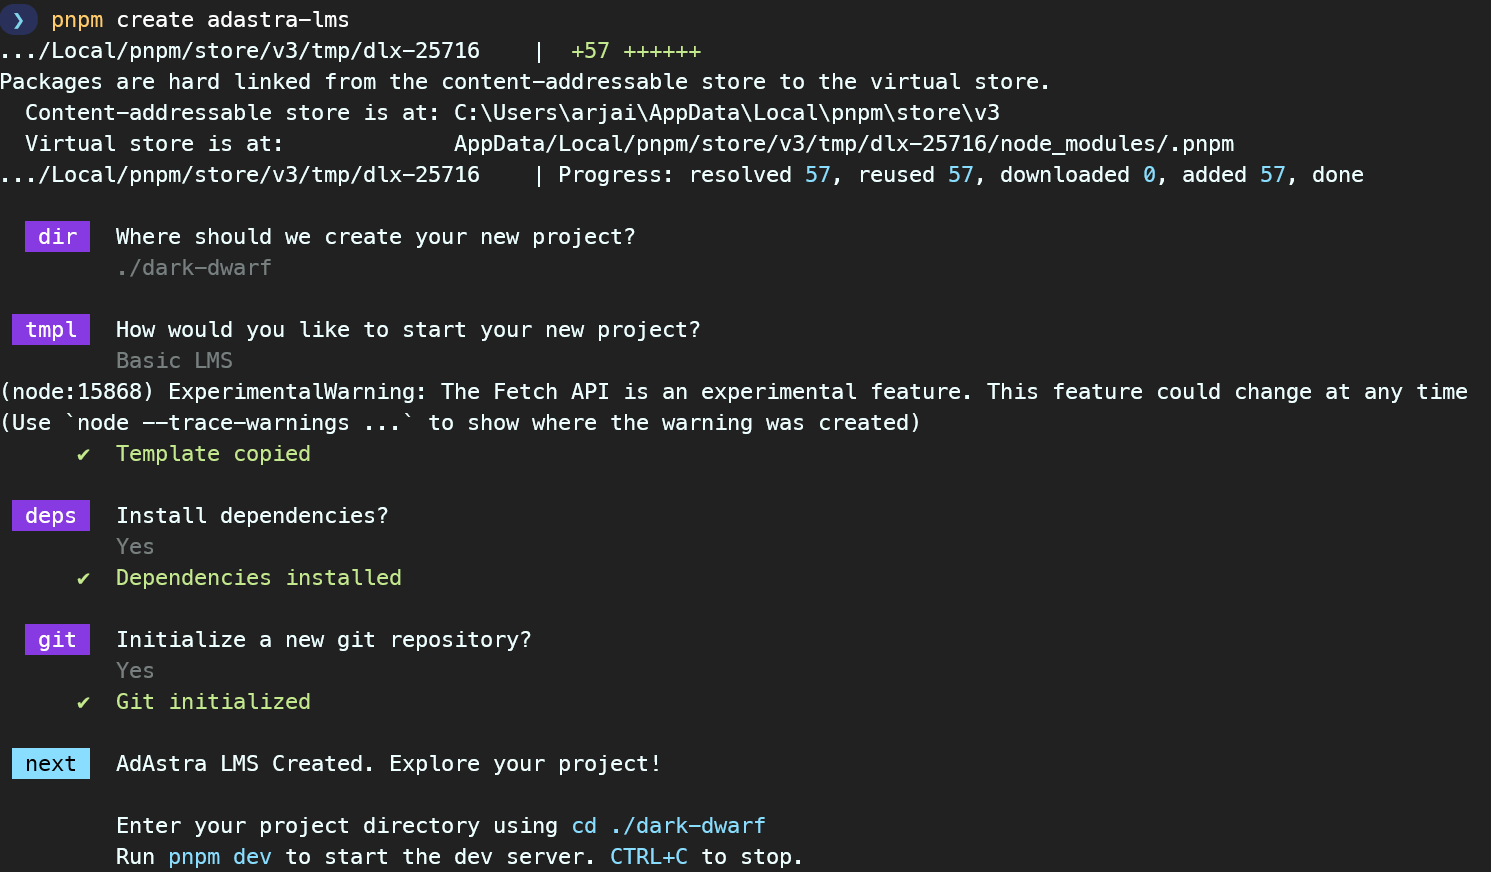
\includegraphics[width=\textwidth]{images/create-adastra-end.png}}
    \caption{Pasos de la ejecución del paquete create-adastra-lms}
    \label{fig:create-adastra}
\end{figure}

Tras usar este comando se creará un proyecto con la estructura mostrada en la figura \ref{fig:adastra-structure}.

\begin{figure}[H]
    \centering
    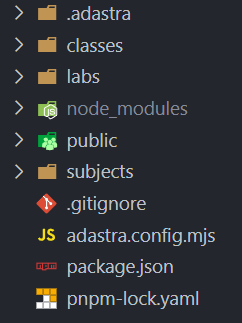
\includegraphics{images/projectStructure.png}
    \caption{Estructura de un proyecto creado con create-adastra-lms}
    \label{fig:adastra-structure}
\end{figure}

\section{Configuración del LMS}
El primer paso a seguir tras crear el proyecto será configurarlo. Hay dos pasos a seguir, 
primero actualizar el archivo de configuración de adastra (\verb|adastra.config.mjs|) y segundo
añadir las variables de entorno necesarias para el proyecto. Un ejemplo del archivo \verb|adastra.config.mjs| sería el que muestra en la figura \ref{fig:adastraConfig}

\subsection{Archivo de configuración: {\tt adastra.config.mjs}}

 Para esto habrá que modificar el archivo \textbf{adastra.config.js} que se ha creado automáticamente. Dentro de este se podrán encontrar dos objetos, el primero llamado \textbf{tailwindConfig} que se puede ver en la figura \ref{fig:adastraConfig} en la linea 1, el cual permitirá cambiar configuraciones relacionadas con el tema de la página que se creará como los colores primarios y secundarios, teniendo cada uno su opción para el estilo oscuro de la página, o incluso el tamaño que asignar al espaciado mínimo o la altura del navbar, etc. Esto funciona con la configuración de tailwindcss como base, en la documentación de tailwindcss (\cite{tailwind-theme}) se puede encontrar más información sobre esto. Y un segundo, llamado \textbf{organizationInfo} que se puede ver en la figura \ref{fig:adastraConfig} en la linea 24, dentro de este habrá que aportar información relacionada con la organización. Entre ellos los datos más importantes a introducir serían los siguientes:

 \begin{itemize}
    \item \textbf{pageTitle:} Titulo que aparecerá en la aplicación
    \item \textbf{github:} Objeto de configuración sobre GitHub
        \begin{itemize}
            \item \textbf{organizationName(obligatorio):} El nombre de la organización en GitHub.
            \item \textbf{classroomUrl:} Url del Classroom creado anteriormente.
        \end{itemize}
    \item \textbf{virtualCampus:} Objeto de configuración sobre el campus virtual
        \begin{itemize}
            \item \textbf{teachingGuideUrl:} Url a la guia docente de la asignatura
            \item \textbf{campusUrl:} Url al campus virtual de la asignatura
            \item \textbf{labsUrl:} Url a las tareas de la asignatura
        \end{itemize}
\end{itemize}

\begin{figure}
  \begin{lstlisting}[language=Javascript]
        export const tailwindConfig = {
          theme: {
            extend: {
              colors: {
                primary: "rgb(51 153 255 / <alpha-value>)",
                "dark-primary": "rgb(51 153 255 / <alpha-value>)",
                secondary: "rgb(135 45 230 / <alpha-value>)",
                "dark-secondary": "rgb(135 45 230 / <alpha-value>)",
                ...
              },
              spacing: {
                "navbar-height": "6rem",
                "sidebar-width": "18rem",
                ...
              },
              fontSize: {
                code: "1rem",
                ...
              },
            },
          },
        };
        
        export const organizationInfo = {
          pageTitle: "Test Asignatura",
          github: {
            organizationName: "ULL-ESIT-PL-2122",
            classroomUrl: "",
          },
          virtualCampus: {
            teachingGuideUrl: "",
            campusUrl: "",
            labsUrl: "",
          },
        };
    \end{lstlisting}
    \caption{Ejemplo del archivo de configuración de AdAstra: adastra.config.mjs}
    \label{fig:adastraConfig}
\end{figure}

\subsection{Configurar las variables de entornos}

Además para que la aplicación pueda obtener datos de la organización desde la API GraphQL de GitHub se tendrá que añadir a las variables de entorno del programa un token de acceso personal de GitHub \url{github-token}, llamándolo \textbf{GITHUB\_SECRET}, en la figura\ref{fig:scopes} se muestra los \verb|scopes| que necesitará el token. La manera normal de añadir este secreto es a través de un \verb|.env| en el desarrollo y a la hora de hacer el despliegue de la aplicación habría que añadirlo a las variables de entorno del servicio. Por ejemplo, si se usa \verb|Vercel| \cite{vercel} como plataforma para el despliegue de la aplicación en la sección de \textit{Settings} hay un apartado llamado 
\textit{Environment Variables} en el que se pueden añadir variables de entornos a la aplicación. En la figura \ref{fig:vercelEnv} se puede ver de forma más detallada este menú.

\begin{figure}[H]
    \centering
    \makebox[\textwidth][c]{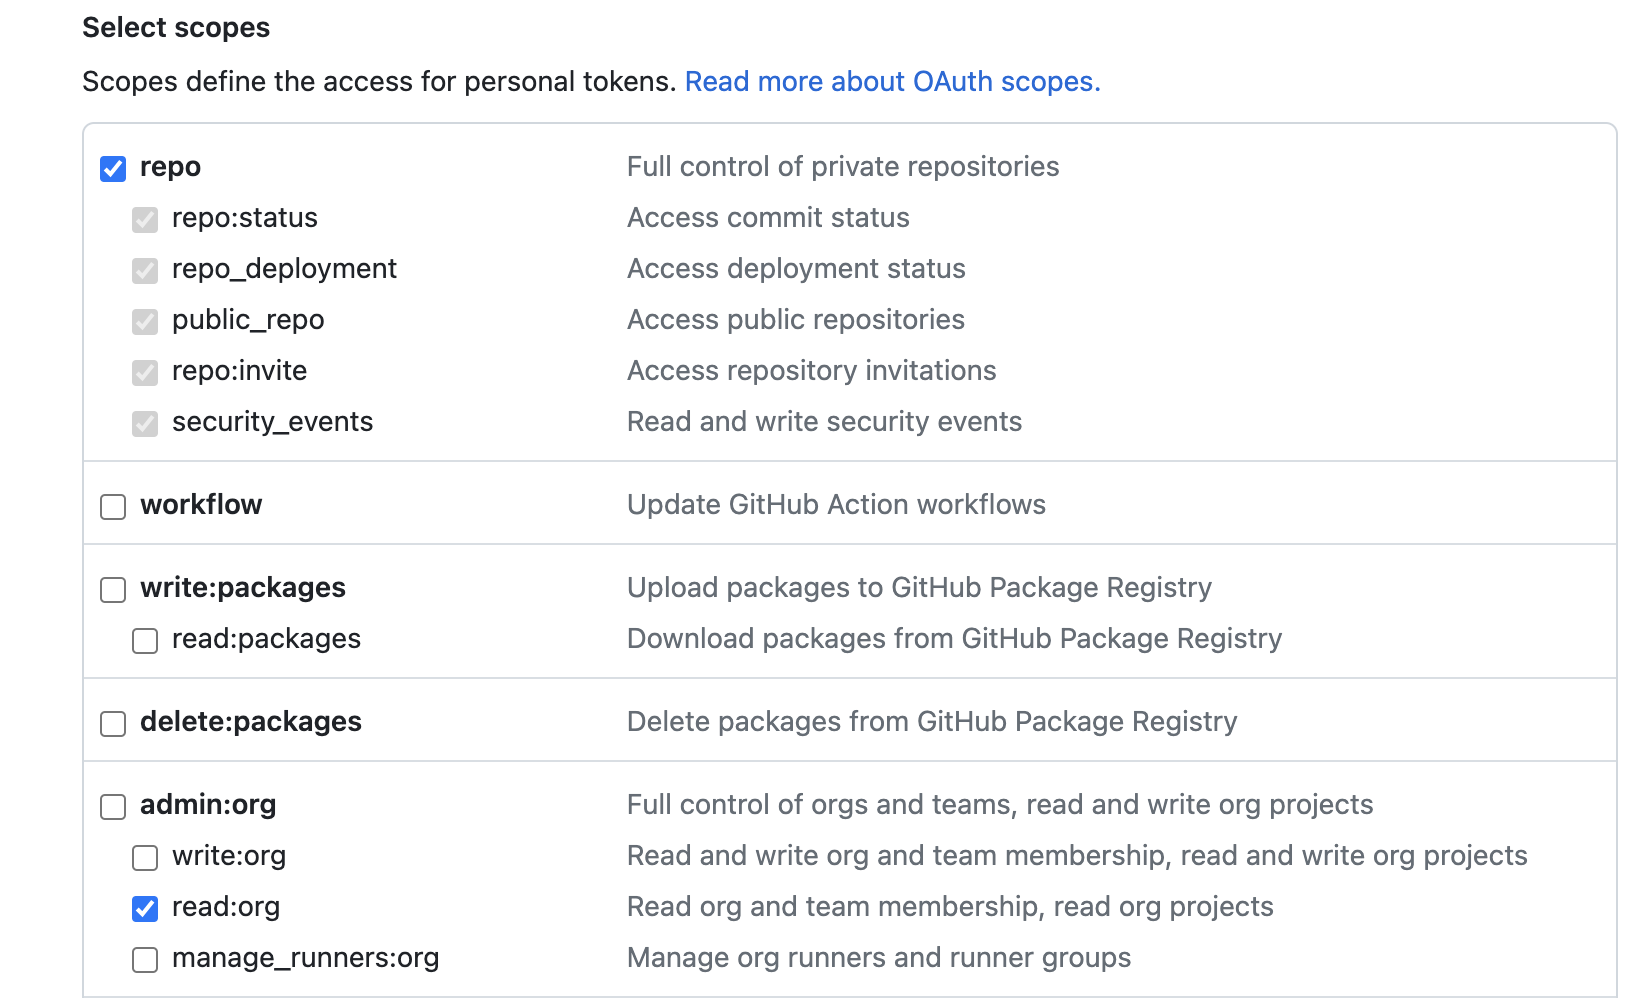
\includegraphics[width=\textwidth]{images/scopes.png}}
    \caption{Scopes para el token GITHUB\_SECRET}
    \label{fig:scopes}
\end{figure}

Ahora que ya está configurado podremos iniciar el proyecto localmente con el comando:
\begin{verbatim}
    npm run dev
\end{verbatim}

\begin{figure}[H]
    \centering
    \makebox[\textwidth][c]{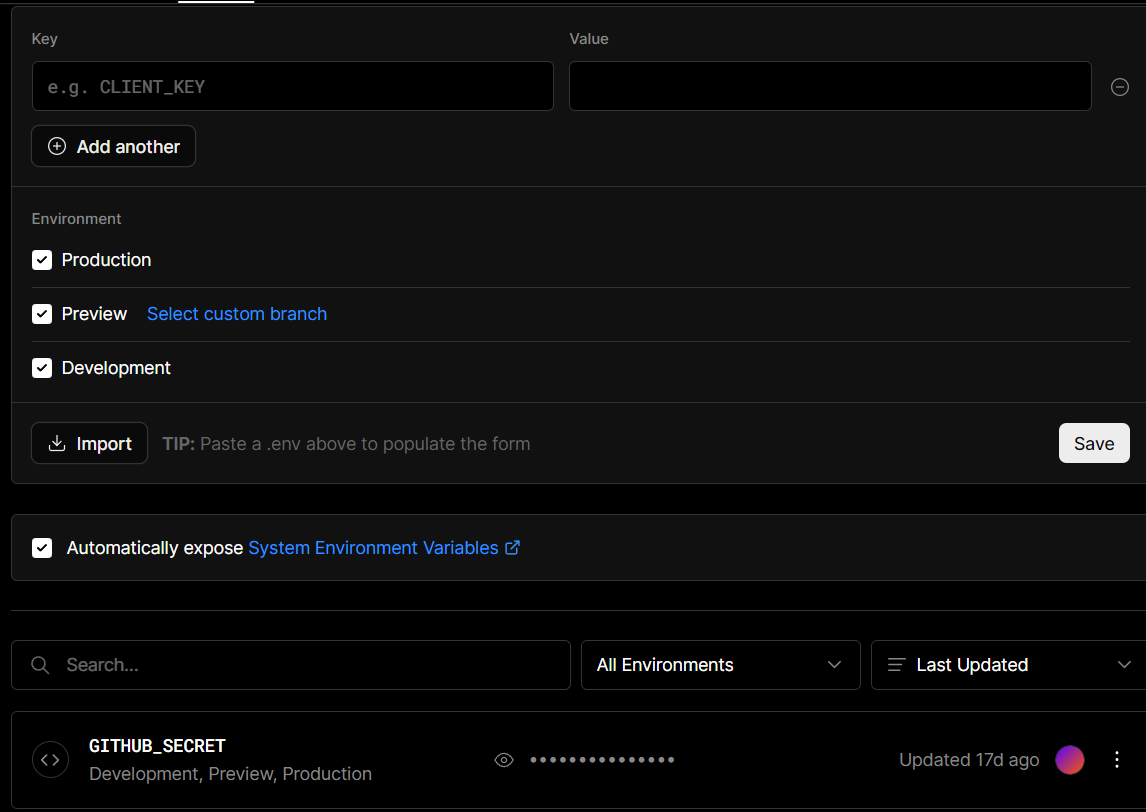
\includegraphics[width=\textwidth]{images/vercelEnv.png}}
    \caption{Menú para las variables de entorno en Vercel}
    \label{fig:vercelEnv}
\end{figure}

\section{Añadir contenido al LMS}

En cuanto al contenido habrá que diferenciar en cuatro tipos, elementos generales que se comparten entre todos los contenidos como imágenes, vídeos, archivos, etc; prácticas(\verb|labs|), temarios(\verb|subjects|) y clases(\verb|classes|).

\subsection{Contenido general: {\tt public}}

El primer tipo de contenido, como se dijo anteriormente están relacionados con elementos que se quiera acceder en el resto de manera general, un ejemplo una imagen, y de base no modifican la pagina web que se crea, sino que sirven para expandir el tipo de información a poder usar en los contenidos posteriores. Por esto se proporciona una carpeta llamada \textbf{public}. Para poder acceder a estos elementos a posterior, se deberán usar accesos absolutos respecto a la carpeta public. Unos ejemplos serían estos:

\begin{verbatim}
    public/test.png -> /test.png
    public/images/test.png -> /images/test.png
\end{verbatim}

\subsection{Añadir un temario}

El primer contenido que deberá ser escrito por el usuario directamente y que realizará un cambio explicito en la aplicación serán los temarios, que están ubicados en la carpeta \textbf{subjects}. Para añadir una nueva entrada se deberá crear un archivo de tipo \verb|Markdown| \cite{md}. Se deberá tener en cuenta que la aplicación usa un sistema de navegación automático basado en el nombre de los archivos, por esto se deberá añadir un numero antes del nombre del archivo. Un ejemplo es este:

\begin{verbatim}
    test-subject.md -> 1-test-subject.md
\end{verbatim}

Además, el nombre del archivo deberá estar con \verb|-| como separador y tener en cuenta que el nombre del elemento en la navegación irá en función del nombre del archivo.

\begin{verbatim}
    1-test-subject.md -> Test Subject
\end{verbatim}

Dentro de estos archivos habrá que añadir contenido como se trabaja de normal con los archivos markdown, aunque se deberá escribir un contenido extra llamado \textbf{fromatter} al principio del archivo que permitirá darle información importante al generador. Un ejemplo de como se ve en \textbf{subjects} es este:

\begin{verbatim}
    ---
    type: subject
    description: "hello world test"
    title: "Getting Started"
    key: getting-started
    ---
\end{verbatim}

La explicación de cada uno es la siguiente:

\begin{itemize}
    \item \textbf{type:} En los temarios se deberá poner siempre \verb|subject|.
    \item \textbf{description:} Descripción general del archivo.
    \item \textbf{title:} Será el título que tendrá esa entrada al generarse.
    \item \textbf{key:} Clave con la que se identificará al archivo en el proyecto.
\end{itemize}

\subsection{Añadir una práctica}

Este contenido funcionará igual que el anterior, pero está relacionado con un tarea o práctica de la asignatura. Hay que destacar que en el frontmatter se proporcionará un \textit{key} para relacionar esta práctica con la creada en el Classroom de Github, esto se usará en la construcción de la información de los alumnos en el apartado de prácticas de cada uno. Un ejemplo de como se ve el frontmatter de los \textbf{labs} es este:

\begin{verbatim}
    ---
    type: lab
    title: Egg Parser
    key: egg-parser
    templateKey: egg-parser-template
    ---
\end{verbatim}

La explicación de cada uno es la siguiente:

\begin{itemize}
    \item \textbf{type:} En las prácticas se deberá poner siempre \verb|lab|.
    \item \textbf{title:} Será el título que tendrá esa entrada al generarse.
    \item \textbf{key:} Clave con la que se identificará al archivo en el proyecto.
    \item \textbf{templateKey:} Clave de la template del lab en la organización de GitHub creado por el Classroom de GitHub que se relacionará con este archivo, en este caso sería el nombre del repositorio de la template.
\end{itemize}

\subsection{Añadir una clase}

Al igual que los anteriores se usará markdown para añadir una clase. Hay que destacar que en el frontmatter se deberá proporcionar una lista de \textbf{labs} y \textbf{subjects} relacionados, para que se genere de manera automática los links a estos en la entrada generada en la aplicación.
Un ejemplo de como se ve el frontmatter de las \textbf{classes} es este:

\begin{verbatim}
    ---
    type: class
    title: Lunes 2023/05/08
    relatedLabs:
      - egg-parser
    relatedSubjects:
      - getting-started
    ---
\end{verbatim}

La explicación de cada uno es la siguiente:

\begin{itemize}
    \item \textbf{type:} En los clases se deberá poner siempre \verb|class|.
    \item \textbf{title:} Será el título que tendrá esa entrada al generarse.
    \item \textbf{relatedLabs:} Lista de las claves de los labs a relacionar con está clase.
    \item \textbf{relatedSubjects:} Lista de las claves de los subjects a relacionar con está clase.
\end{itemize}

\section{Hacer un despliegue del LMS}

Para hacer un despliegue se deberá escoger donde querremos que se haga, pero para este ejemplo usaremos el hosting de vercel como ejemplo, aunque el resto de casos deberá ser parecido.

Lo primero será crearse una cuenta de vercel, como tienen para usar GitHub como cuenta usaremos está opción para simplificar el proceso. Tras esto se nos abrirá un panel como el de la figura \ref{fig:vercelPanel}, dentro de este seleccionaremos \textit{Add New -> Project}. Esto nos abrirá una nueva página como la figura \ref{fig:vercelNewProject}, en este caso vercel funciona usando los repositorios de GitHub del usuario como posibles proyectos, deberemos seleccionar el proyecto que queramos desplegar. Esto abrirá un panel para configurar el proyecto como el de la figura \ref{fig:vercelConfig}, deberemos introducir los siguientes datos:

\begin{itemize}
    \item \textbf{Project Name:} El nombre que queremos usar en vercel.
    \item \textbf{Build Command:} Será el comando que sirva para construir la app: 
        \begin{verbatim}
            npm run dev
        \end{verbatim}
    \item \textbf{Enviroment Variables:} Aquí se deberá añadir la variable de entorno \verb|GITHUB_SECRET| con el token de GitHub creado anteriormente.
\end{itemize}

\begin{figure}
    \centering
    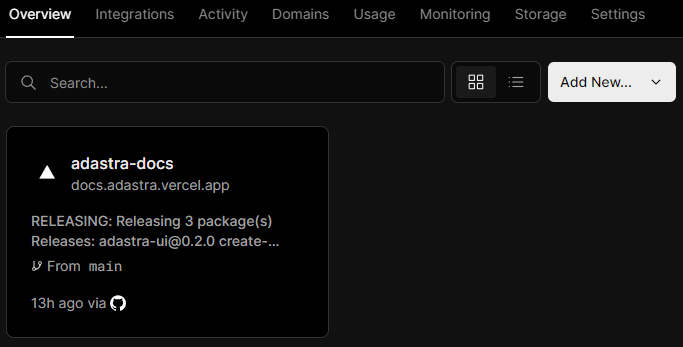
\includegraphics{images/vercelPanel.png}
    \caption{Panel principal de Vercel}
    \label{fig:vercelPanel}
\end{figure}

\begin{figure}
    \centering
    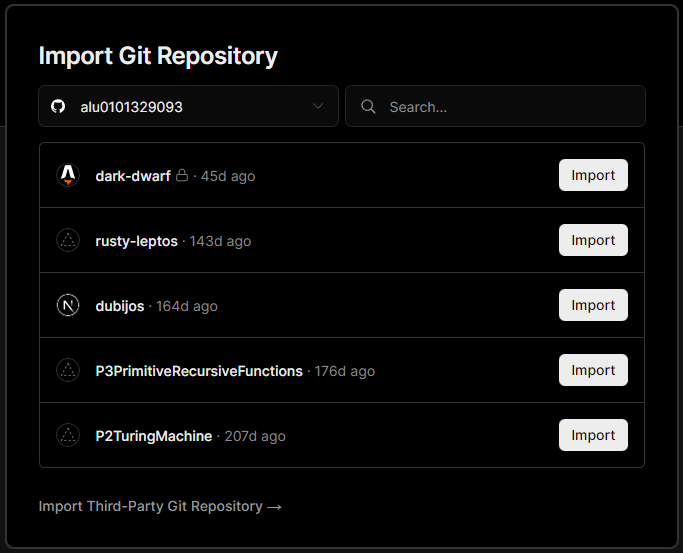
\includegraphics{images/vercelNewProject.png}
    \caption{Panel para añadir un nuevo proyecto en Vercel}
    \label{fig:vercelNewProject}
\end{figure}

\begin{figure}
    \centering
    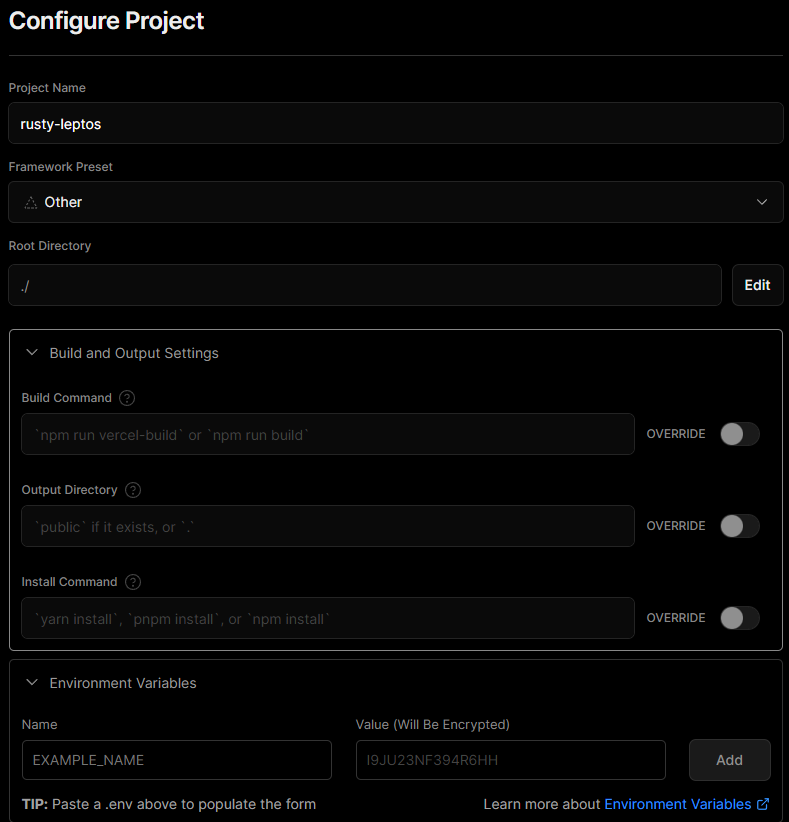
\includegraphics[scale=0.8]{images/vercelConfig.png}
    \caption{Panel de configuración del nuevo proyecto en Vercel}
    \label{fig:vercelConfig}
\end{figure}